
\documentclass[10pt]{article}
\usepackage[utf8]{inputenc}
\usepackage{graphicx}
\usepackage{amsmath, amssymb}
\usepackage{geometry}
\usepackage{caption} 
\geometry{a4paper, margin=0.5in, landscape} 

\begin{document}

\section*{Comparative EIS Kinetics Report}
\textbf{Model Structure:} \texttt{R0-p(R1-p(R2,CPE2),CPE1)}

\begin{center}
    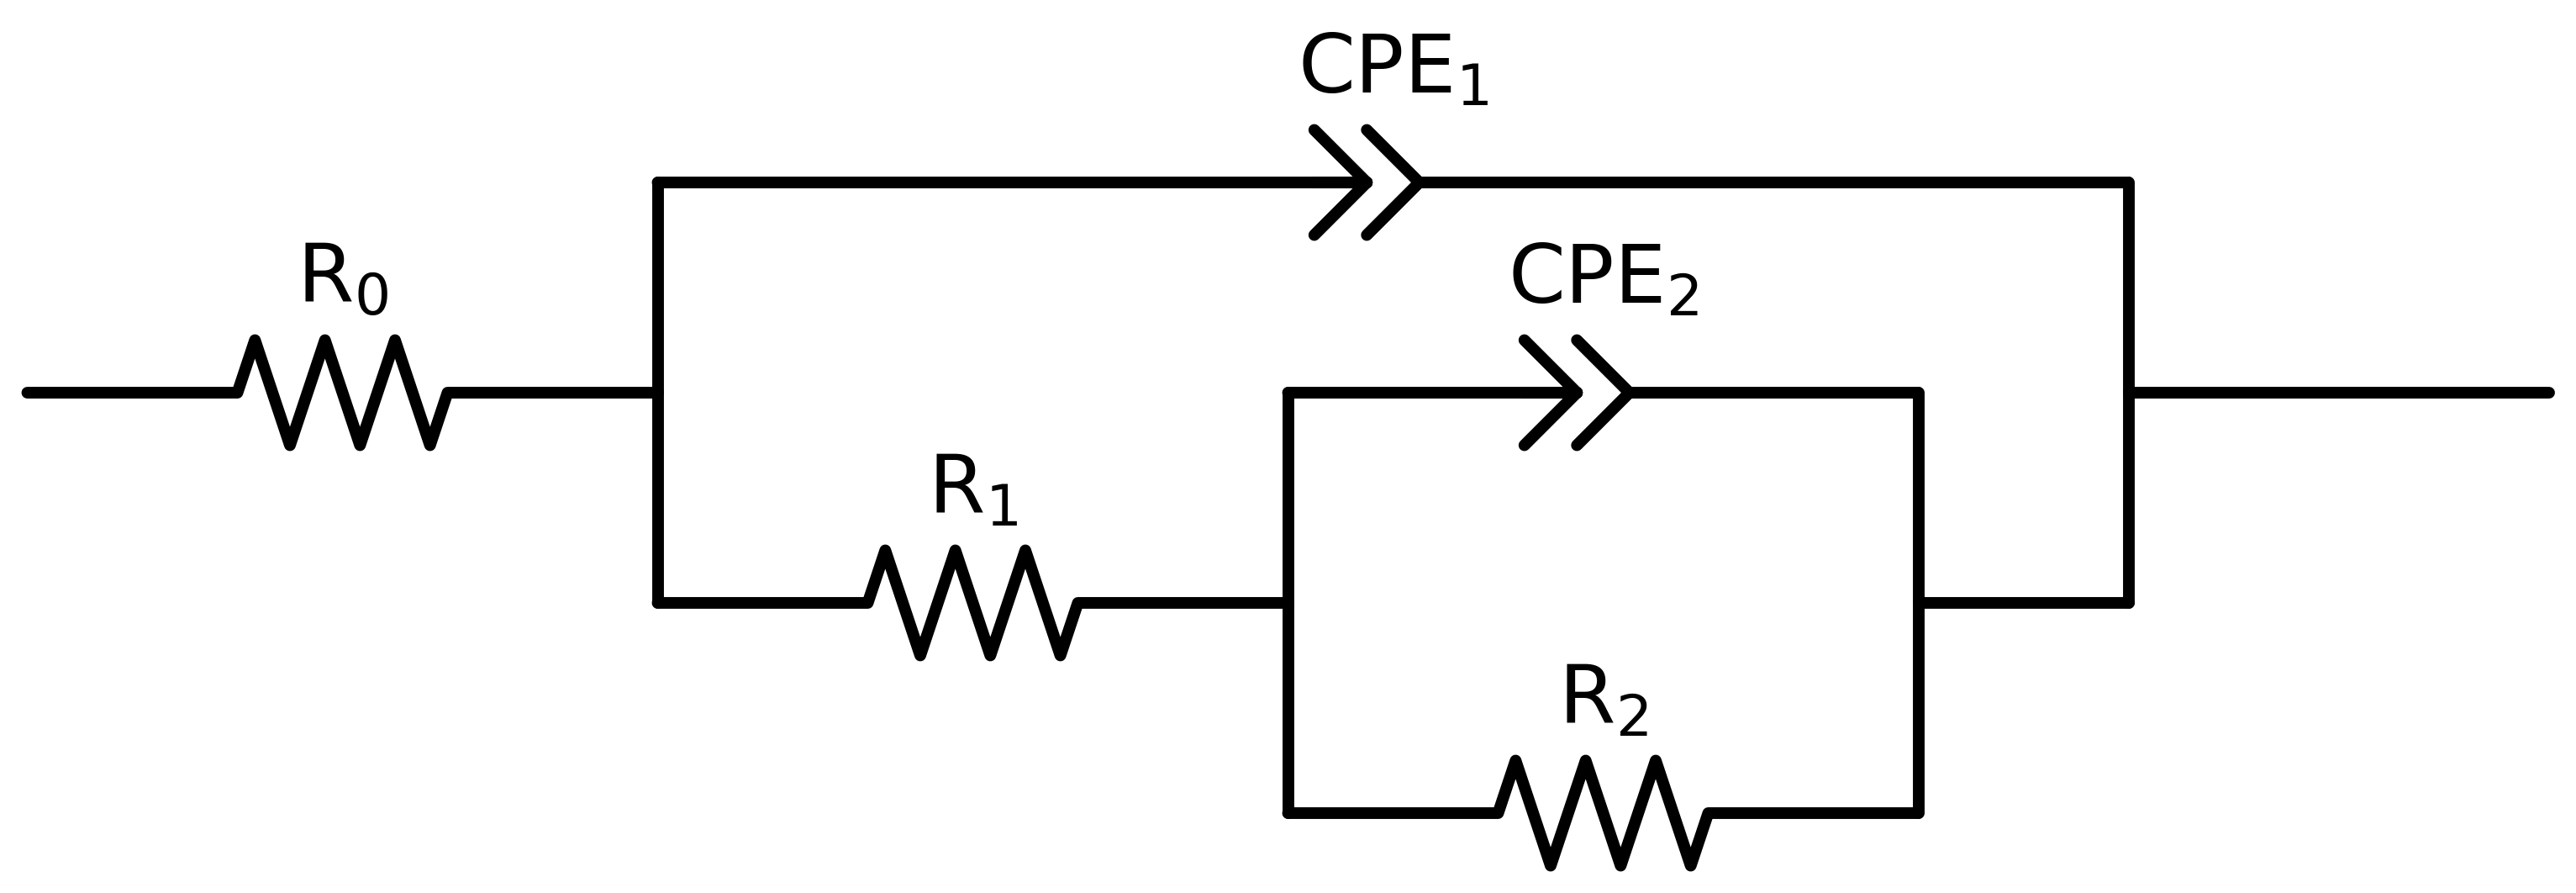
\includegraphics[width=0.45\textwidth]{../../2RC.png}
\end{center}

\renewcommand{\arraystretch}{1.6} 
\begin{table}[h!]
    \centering
    \footnotesize
    \begin{tabular}{|l|c|c|c|c|c|c|c|}
        \hline
        \textbf{Element} & \textbf{Unit} & \textbf{Bounds} & \textbf{Cauvel\_4\_NaCl\_8H} & \textbf{Cauvel\_4\_NaCl\_24H} & \textbf{Cauvel\_4\_NaCl\_48H} & \textbf{Cauvel\_4\_NaCl\_72H} & \textbf{Cauvel\_4\_NaCl\_168H} \\ \hline
        $R_{0}$ & $\Omega$ & $[1.0e-03, 1.0e+03]$ & $7.56e+01 \pm 7.5e-01$ & $7.23e+01 \pm 3.2e-01$ & $7.06e+01 \pm 3.2e-01$ & $5.48e+00 \pm 3.7e+03$ & $5.36e+01 \pm 2.7e-01$ \\ \hline
        $R_{1}$ & $\Omega$ & $[1.0e+00, 1.0e+08]$ & $1.42e+01 \pm 6.1e+03$ & $3.91e+03 \pm 9.5e+02$ & $3.80e+03 \pm 5.3e+02$ & $5.82e+01 \pm 3.7e+03$ & $4.21e+03 \pm 2.8e+02$ \\ \hline
        $R_{2}$ & $\Omega$ & $[1.0e+00, 1.0e+08]$ & $2.41e+04 \pm 6.3e+03$ & $2.91e+04 \pm 4.2e+03$ & $2.90e+04 \pm 3.1e+03$ & $2.17e+04 \pm 1.0e+03$ & $1.50e+04 \pm 1.2e+03$ \\ \hline
        $Q_{2}$ & $\Omega$$^{-1}$ sec$^{a}$ & $[1.0e-11, 1.0e-03]$ & $8.03e-05 \pm 5.2e-05$ & $1.39e-04 \pm 1.5e-05$ & $1.78e-04 \pm 1.2e-05$ & $2.03e-04 \pm 4.2e-06$ & $3.94e-04 \pm 3.1e-05$ \\ \hline
        $n_{2}$ & - & $[5.0e-01, 1.0e+00]$ & $5.00e-01 \pm 4.5e-02$ & $5.00e-01 \pm 4.5e-02$ & $5.82e-01 \pm 3.5e-02$ & $7.44e-01 \pm 6.2e-03$ & $7.72e-01 \pm 3.6e-02$ \\ \hline
        $Q_{1}$ & $\Omega$$^{-1}$ sec$^{a}$ & $[1.0e-11, 1.0e-03]$ & $5.03e-05 \pm 3.0e-05$ & $9.94e-05 \pm 3.8e-06$ & $1.06e-04 \pm 3.4e-06$ & $1.79e-09 \pm 1.1e-07$ & $1.60e-04 \pm 3.5e-06$ \\ \hline
        $n_{1}$ & - & $[5.0e-01, 1.0e+00]$ & $8.97e-01 \pm 1.3e-01$ & $8.35e-01 \pm 6.9e-03$ & $8.57e-01 \pm 6.3e-03$ & $9.06e-01 \pm 5.4e+00$ & $8.60e-01 \pm 5.0e-03$ \\ \hline
        \textbf{$\chi^2$} & - & -  & $8.056e-04$ & $4.777e-04$ & $5.433e-04$ & $5.893e-03$ & $7.207e-04$ \\ \hline

    \end{tabular}
\end{table}


\newpage
\section*{Analysis Results: 8H}
\begin{center}
    
\includegraphics[width=0.7\textwidth]{plots_Cauvel_4_NaCl_8H.pdf}
    \captionof{figure}{EIS Fit Results for Cauvel\_4\_NaCl\_8H}
\end{center}

\newpage
\section*{Analysis Results: 24H}
\begin{center}
    
\includegraphics[width=0.7\textwidth]{plots_Cauvel_4_NaCl_24H.pdf}
    \captionof{figure}{EIS Fit Results for Cauvel\_4\_NaCl\_24H}
\end{center}

\newpage
\section*{Analysis Results: 48H}
\begin{center}
    
\includegraphics[width=0.7\textwidth]{plots_Cauvel_4_NaCl_48H.pdf}
    \captionof{figure}{EIS Fit Results for Cauvel\_4\_NaCl\_48H}
\end{center}

\newpage
\section*{Analysis Results: 72H}
\begin{center}
    
\includegraphics[width=0.7\textwidth]{plots_Cauvel_4_NaCl_72H.pdf}
    \captionof{figure}{EIS Fit Results for Cauvel\_4\_NaCl\_72H}
\end{center}

\newpage
\section*{Analysis Results: 168H}
\begin{center}
    
\includegraphics[width=0.7\textwidth]{plots_Cauvel_4_NaCl_168H.pdf}
    \captionof{figure}{EIS Fit Results for Cauvel\_4\_NaCl\_168H}
\end{center}


\end{document}
